\subsection{MATH-500}
{{\footnotesize
\noindent MATH-500 is a curated subset of 500 problems from the OpenAI MATH dataset, spanning
high-school to advanced levels, designed to evaluate LLMs mathematical reasoning and 
generalization.


\begin{description}[labelwidth=4cm, labelsep=1em, leftmargin=4cm, itemsep=0.1em, parsep=0em]
  \item[date:] 2025-02-15
  \item[version:] 1
  \item[last\_updated:] 2025-02-15
  \item[expired:] false
  \item[valid:] yes
  \item[valid\_date:] 2025-02-15
  \item[url:] \href{https://huggingface.co/datasets/HuggingFaceH4/MATH-500}{https://huggingface.co/datasets/HuggingFaceH4/MATH-500}
  \item[doi:] unknown
  \item[domain:] Mathematics
  \item[focus:] Math reasoning generalization
  \item[keywords:]
    - calculus
    - algebra
    - number theory
    - geometry
  \item[licensing:] MIT License
  \item[task\_types:]
    - Problem solving
  \item[ai\_capability\_measured:]
    - Math reasoning and generalization
  \item[metrics:]
    - Accuracy
  \item[models:]
    - unkown
  \item[ml\_motif:]
    - Math problem solving
  \item[type:] Benchmark
  \item[ml\_task:]
    - Supervised Learning
  \item[solutions:] 0
  \item[notes:] Dataset hosted on Hugging Face. Data comes from a subset of OpenAI's dataset
  \item[contact.name:] unknown
  \item[contact.email:] unknown
  \item[datasets.links.name:] Hugging Face
  \item[datasets.links.url:] \href{https://huggingface.co/datasets/HuggingFaceH4/MATH-500}{https://huggingface.co/datasets/HuggingFaceH4/MATH-500}
  \item[results.links.name:] unknown
  \item[results.links.url:] \href{unknown}{unknown}
  \item[fair.reproducible:] True
  \item[fair.benchmark\_ready:] True
  \item[id:] math-
  \item[Citations:] \cite{huggingface2025math500}
\end{description}

{\bf Ratings:} ~ \\

\begin{tabular}{p{0.15\textwidth} p{0.07\textwidth} p{0.7\textwidth}}
\hline
Rating & Value & Reason \\
\hline
dataset & 5 & Problems and solutions are easily downloaded. Could not find a way to download the data
 \\
documentation & 0 & Not given. Implicit instructions to download dataset.
 \\
metrics & 2 & Problem spec states that all of the AI reasoning steps are subject to grading, but no specified way to evaluate the steps
 \\
reference\_solution & 0 & Not given
 \\
software & 0 & No code provided
 \\
specification & 0 & No method of presentation and evaluation is not stated. No constraints
 \\
\hline
\end{tabular}

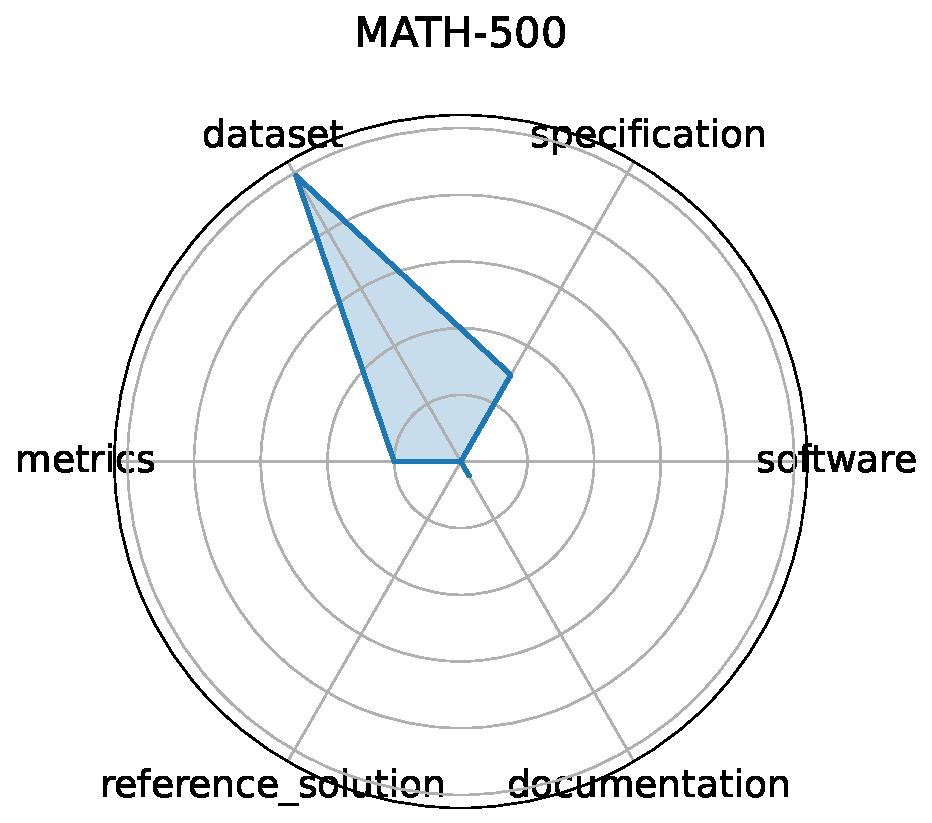
\includegraphics[width=0.2\textwidth]{math-_radar.pdf}
}}
\clearpage